\chapter{Logic II}

\epigraph{Contrariwise, if it was so, it might be; and if it were so, it would be; but as it isn't, it ain't. That's logic.}{Lewis Carroll}

Okay, for people who like videos. \href{https://www.youtube.com/watch?v=cDRqud3q3Fg}{Bian McLogan} has an explination of converse, inverse, and contrapositive. \href{https://www.youtube.com/watch?v=tKnS3s8fOu4}{shaunteaches} has an overview of De Morgan's Laws. \href{https://www.youtube.com/watch?v=YBNrkXEqCiI}{Alicia Gray} has a video on logical arguments. \href{https://www.youtube.com/watch?v=N6_Q1kcXiIg}{Math and Stats Help} has a video on Euler digrams.

Last time we established the basicis of logic using truth tables. We know that basic logical operators, and we can resolve statements using truth tables. This time we will look at how we can apply logical laws to statements, and see their application in circuits.

\section{Converse, Inverse, and Contrapositive of implication}

For a few seconds in class, we ``learned'' in the inverse of implication (incorrectly called ``inverse of a statement''), but I want to go into that in some more detail. Given an implication (if $P$ then $Q$), we can form the {\bf converse}, {\bf inverse}, and {\bf contrapositive}.

\begin{boxdefine}{Converse, Inverse, and Contrapositive of Implication}{}
	Given the statement $P \implies Q$ (if $P$, then $Q$), the following can be defined.
	\begin{itemize}
		\item The {\bf converse} is $Q \implies P$ (if $Q$, then $P$).
		\item The {\bf inverse} is $\lnot P \implies \lnot Q$ (if not $P$, then not $Q$).
		\item The {\bf contrapositive} is $\lnot Q \implies \lnot P$ (if not $Q$, then not $P$).
	\end{itemize}
\end{boxdefine}

Generally I think its better to think about logic in English rather then symbolically. Even if the symbols above look confusing to you, take a look at the examples below in English.

\begin{boxexample}{}{}
	Suppose our implication is ``if you write fanfic, then you're cool.'' Then we have
	
	\begin{itemize}
		\item The converse is ``if you're cool, you write fanfic.''
		\item The inverse is ``if you don't write fanfic, then you're not cool.''
		\item The contrapositive is ``if you're not cool, you don't write fanfic.''
	\end{itemize}
\end{boxexample}

Keep in mind that the converse and inverse aren't nessesarily correct. However, if the statement is correct then the contrapositive is equivalent.

\begin{boxproposition}{Contrapositive of inverse}{}
	Given an implication is true, then the contrapositive is also true, denoted by
	\[
		(A \implies B) \iff (\lnot B \implies \lnot A)
	\]
\end{boxproposition}

We spent 7 seconds on this in class, so I assume its not too important. At the very least, make sure you know how to do inverse of implication. I'm not sure if we'll need to do converse and contrapositive, though they are typically taught togeather and closely related.

\section{De Morgan's Laws}

De Morgan's laws allows the experession of conjunctons and disjunctions purely in terms of each other via negation. Phew, thats a lot of words. Basically, you can use the following laws to simplify negations.

\begin{boxproposition}{De Morgan's Laws}{}
	\[
		\lnot (A \lor B) \iff \lnot A \land \lnot B
	\]
	\[
		\lnot (A \land B) \iff \lnot A \lor \lnot B
	\]
\end{boxproposition}

Again, since this is logic, I recommend considering this in English to understand whats going on. For example,

\begin{boxexample}{}{}
	\begin{itemize}
		\item What is the negation of ``gaming or studying'' Answer: ``Not gaming and not studying.''
		\item What is the negation of ``drinking and driving?'' Answer: ``Not driving or not drinking.''
	\end{itemize}
\end{boxexample}

\section{Arguments in Classical Logic}

Instead of using truth tables to determine that valididity of statements, we can use {\bf arguments}. When we make an argument, we assume some premise and reach a conclusion.

\begin{boxdefine}{Laws of Detachment, Contraposition, Syllogism, and Disjunctive Syllogism}{}
	Here is a list of some true arguments.

	\begin{itemize}
		\item {\bf Law of Detachment}: If $A$ implies $B$, and $A$ is true, then $B$ must be true. Denoted by $(A \implies B) \land A \implies B.$
		\item {\bf Law of Contraposition}: If $A$ implies $B$, and $B$ is false, then $A$ must be false. Denoted by $(A \implies B) \land \lnot B \implies \lnot A.$
		\item {\bf Law of Syllogism}: If $A$ implies $B$, and $B$ implies $C$, then $A$ implies $C$. Denoted by $(A \implies B) \land (B \implies C) \implies (A \implies C).$
		\item {\bf Law of Disjunctive Syllogism}: If $A$ or $B$ are true, but $A$ is false, then $B$ is true. Denoted by $(A \lor B) \land \lnot A \implies B$.
	\end{itemize}
\end{boxdefine}

The notes go onto prove these with truth tables. I think the proofs are too easy though, and that some examples of these in \cancel{English} Minecraft are more useful to you.

\begin{boxexample}{}{}
	\begin{itemize}
		\item {\bf Law of Detachment}: If a creeper destroys my base, then I will build a new base. A Creeper destoyed my base. Therefor, I will build a new base.
		\item {\bf Law of Contraposition}: If a creeper destroys my base, then I will build a new base. I did not build a new base. Therefor, a creeper has not destroyed my base.
		\item {\bf Law of Syllogism}: If a creeper destorys my base, then I will build a new base. If I build a new base, I will collect stone. Therefor, if a creeper destroys my base, I will collect stone.
		\item {\bf Law of Disjunctive Syllogism}: I will build underwater or underground. I am not building underwater. Therefor, I am building underground.
	\end{itemize}
\end{boxexample}

An invalid agrument is called a {\bf fallacy}. It seems for this course we're only going to be using two fallacies.

\begin{boxdefine}{Fallacy of Converse and Inverse}{}
	\begin{itemize}
		\item {\bf Fallacy of Converse}: If $A$ implies $B$, and $B$ is true, then $A$ is true. Denoted by $(A \implies B) \land B \implies A$.
		\item {\bf Fallacy of Inverse}: If $A$ implies $B$, and $A$ is fase, then $A$ is false. Denoted by $(A \implies B) \land \lnot A \implies \lnot B$.
	\end{itemize}
\end{boxdefine}

Tired of this yet? Here's a few more examples of these.

\begin{boxexample}{}{}
	Some examples of fallacies (or invalid arguments) are

	\begin{itemize}
		\item {\bf Fallacy of Converse}: If I am in a cave, I will use a tourch. I am using a torch. Therefor, I am in a cave.
		\item {\bf Fallacy of Inverse}: If I am in a cave, I will use a torch. I am not in a cave. Therefor, I am not using a tourch.
	\end{itemize}
\end{boxexample}

\begin{boxremark*}{}{}
	The logic we're currently doing is called {\bf Propositional Logic}. But there are other systems of logic. For example {\bf Predicate Logic} (also called first-order logic) is the most popular logic system for mathematics. Predicate logic defines two more symbols: ``$\forall$'' meaning ``for all'' and ``$\exists$'' meaning ``there exists.'' For example,
	\[
		\forall x \in \mathbb{R}, \exists y \in \mathbb{R} \ni xy = 1
	\]
	reads as ``for all real numbers $x$, there exists real number $y$, such that $ x\cdot y=1.$ There is one other important thing that you might want to know about logic, especially if you're interested in Artificial Intellegence. The systems presented to you in this course are languages. Languages alone aren't too useful. What mathematitions do to make logic useful is define {\bf axioms} (arguments defined to be true) in order to make {\bf deductions}. The laws above are a very weak form of axiom system. A more complete system would be the {\bf Hilbert system}. The first {\bf G\"odel's incompleteness theorem} places restrictions on how complete a consistent system may be.
\end{boxremark*}

\section{Euler Diagrams}

Euler diagrams can be used to express relations between things. For example, if you ever wondered what how the British Isles are classified, look at this interesting CC0 digram I found on Wikipedia.

\includegraphics[scale=0.5]{euler_diagram}

Euler diagrams can also be used to explain logical relations. These are sort of hard to explain, but take a look at the examples below.

\begin{boxexample}{}{}
	Determine if this logic is valid. All students drink alcohol. Scott drinks alcohol. Therefor, Scott is a student.

	Solution: We know that Students drink Alcohol, so we put students inside of an Alcohol circle. We know that Scott drinks alcohol, so we put Scott inside of the alcohol circle along side the students. Thus our diagram looks like this: 

	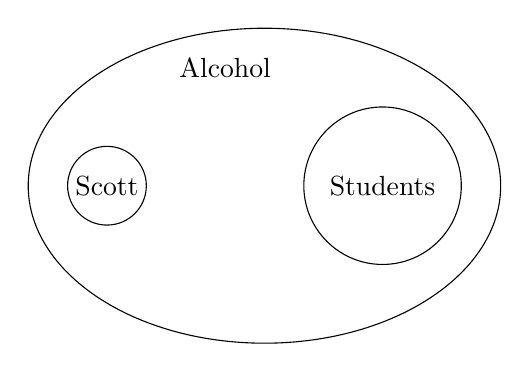
\begin{tikzpicture}
		\draw (0,0) ellipse (3 and 2);
		\node at (-.5,1.5) {Alcohol};
		\draw (1.5,0) circle (1);
		\node at (1.5,0) {Students};
		\draw (-2, 0) circle (0.5);
		\node at (-2,0) {Scott};
	\end{tikzpicture}

	This logic is invalid.
\end{boxexample}

\begin{boxexample}{}{}
	Determine if this logic is valid. All salespeople are annoying. Kelly is a salesperson. Therefor, Kelly is annoying.

	Solution: We know that salespeople are annoying, so we put salepeople inside of the annoying circle. We know that Kelly is a salesperson, so we put Kelly inside of the Salespeople circle. So we have:

	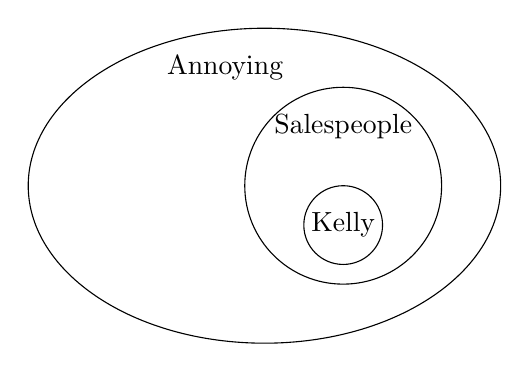
\begin{tikzpicture}
		\draw (0,0) ellipse (3 and 2);
		\node at (-.5,1.5) {Annoying};
		\draw (1,0) circle (1.25);
		\node at (1,0.75) {Salespeople};
		\draw (1,-.5) circle (0.5);
		\node at (1,-.5) {Kelly};
	\end{tikzpicture}

	This logic is valid.
\end{boxexample}

\begin{boxexample}{}{}
	Determine if this logic is valid. All teachers are nice. John is not nice. Therefor, John is not a teacher.

	Solution: We know that teacher are nice, so we put teachers in the nice cirlce. John is not nice, so we put him outside of the nice circle. So we have:

	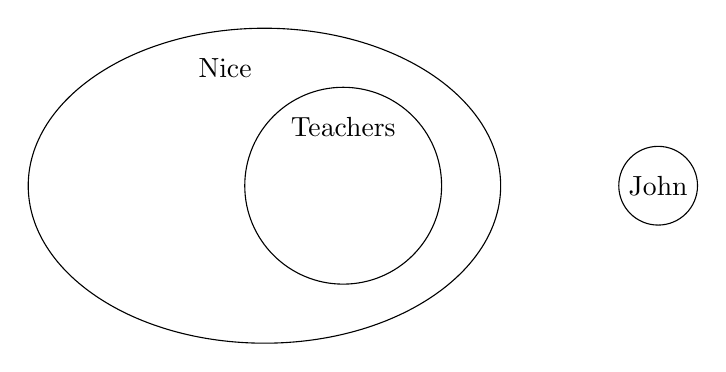
\begin{tikzpicture}
		\draw (0,0) ellipse (3 and 2);
		\node at (-.5,1.5) {Nice};
		\draw (1,0) circle (1.25);
		\node at (1,0.75) {Teachers};
		\draw (5,0) circle (0.5);
		\node at (5,0) {John};
	\end{tikzpicture}

	This logic is valid.
\end{boxexample}


\section{Circuits}

Logic can be used to build circuits. Actually, you can build an entire computer with logic! Such a computer can be built using real-life logic gates, or even built with Redstone in Minecraft! If you're interested in this, I strongly recommend the book \emph{Digital Design and Computer Architecture} by David Money Harris and Sarah L. Harris. In this class, we will look at very simple and/or circuits using switches.

Basically, when we have two switches in parallel, current will run if either of the switches are on. Thus, two switches in parallal are OR ($\lor$).

\begin{boxdefine}{OR Circuit}{}
	$A \lor B$ in circuitry can be defined as

	\begin{circuitikz}
		\draw (0,0)
		to [short, *-] (1,0)
		to [short] (1,1)
		to [short] (2,1)
		to [nos, l=A] (3,1)
		to [short] (4,1)
		to [short] (4,0)
		to [short, -*] (5,0)
		(1,0)
		to [short] (1,-1)
		to [short] (2,-1)
		to [nos, l=B] (3,-1)
		to [short] (4,-1)
		to [short] (4,0);
	\end{circuitikz}
\end{boxdefine}

Then, when we have two switches in series, we need both of them to be on in order for current to flow. So switches in series are AND ($\land$).

\begin{boxdefine}{AND Circuit}{}
	$A \land B$ in circuity can be defined as

	\begin{circuitikz}
		\draw (0,0)
		to [short, *-] (1,0)
		to [nos, l=A] (2,0)
		to [short] (3,0)
		to [nos, l=B] (4,0)
		to [short, -*] (5,0);
	\end{circuitikz}
\end{boxdefine}

Using these building blocks, its possible to write some logical statements as circuits.

\begin{boxexample}{}{}
	The following circuit can be written as $((P \land Q) \lor R) \land S$.

	\begin{circuitikz}
		\draw (0,0)
		to [short, *-] (1,0)
		to [short] (1,1)
		to [short] (2,1)
		to [nos,l=P] (3,1)
		to [short] (4,1)
		to [nos,l=Q] (5,1)
		to [short] (6,1)
		to [short] (6,0)
		to [short] (7,0)
		to [nos,l=S] (8,0)
		to [short,-*] (9,0)
		(1,0)
		to [short] (1,-1)
		to [short] (2,-1)
		to [nos,l=R] (3,-1)
		to [short] (6,-1)
		to [short] (6,0);
	\end{circuitikz}
\end{boxexample}
